\chapter{Hardware moteur}

\section{Cahier des charges du mouvement}

Pour mouvoir le télescope dans des conditions optimales, il y a des contraintes spécifiques à respecter. Le télescope est un appareil qui se doit d'être très précis. Les mouvements étant assurés par les moteurs, il faut que ces derniers soient précis. Les critères à contrôler sont l'angle par pas et le nombre de pas.

Dans un souci de confort d'emploi le télescope doit pouvoir atteindre sa cible sans trop faire patienter l'utilisateur. Il a fallu faire un compromis entre la vitesse et la précision.

\section{Les moteurs}

Nous avons retenu deux type de moteurs~:

\begin{figure}[H]
    \centering
    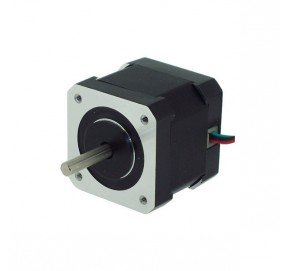
\includegraphics[width=0.49\linewidth]{\figures/photo_motor1.jpg}
    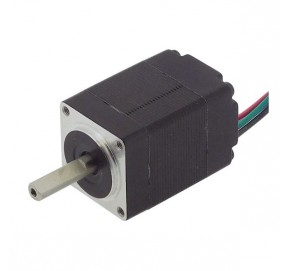
\includegraphics[width=0.3\linewidth]{\figures/photo_motor2.jpg}
    \decoRule
    \caption[
    Moteur 17HM15-0904S et moteur S20STH30-0604A]{
    Moteur 17HM15-0904S et moteur S20STH30-0604A}
    \label{fig:Moteur 17HM15-0904S et moteur S20STH30-0604A}
    \end{figure}

Le premier a été choisi pour l'azimut et l'élévation car il a suffisamment de couple pour mouvoir le télescope, et avec précision. À l'origine, nous en avons trouvé un exemplaire sur les imprimantes 3D et nous avons vérifié s'il répondait à nos contraintes.

Le second est plus léger que le premier, moins puissant. Il est plus adapté pour changer le zoom au bout de la flèche du télescope. Il est indispensable de limiter le poids au bout de la flèche du télescope pour faciliter ses déplacements et surtout ne pas le déséquilibrer.

\section{Le contrôleur}

Le contrôleur est une carte qui à partir de fronts montants en entrée fait tourner un moteur pas à pas d'un angle précis. Cette carte A4988 opto-isolée permet l'entraînement de moteur pas à pas à micropistes Allegro A4988. Il est doté d'une protection contre les surintensités et la surchauffe, ainsi que de cinq résolutions différentes en micropas (jusqu'à 1/16 pas). Il fonctionne de $8V$ à $35V$ et peut fournir jusqu'à environ $1A$ par phase sans dissipateur de chaleur ni flux d'air forcé.

\begin{figure}[H]
    \centering
    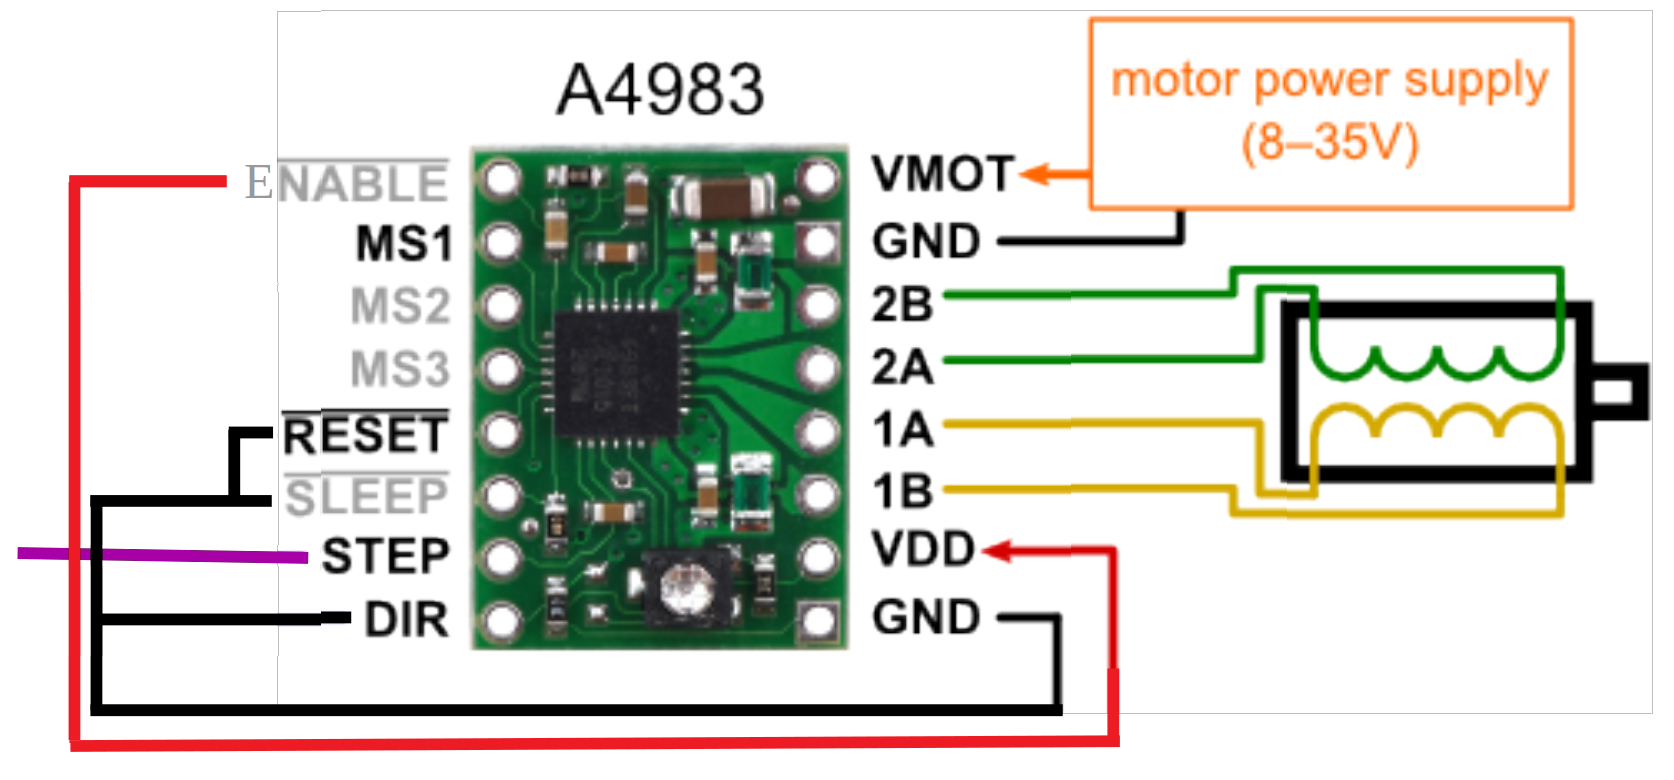
\includegraphics[width=0.6\linewidth]{\figures/sch_a4983.png}
    \decoRule
    \caption[
    Photo du contrôleur A4988]{
    Photo du contrôleur A4988}
    \label{fig:Photo du contrôleur A4988}
    \end{figure}

\section{Validation des moteurs et du câblage}

\begin{figure}[H]
    \centering
    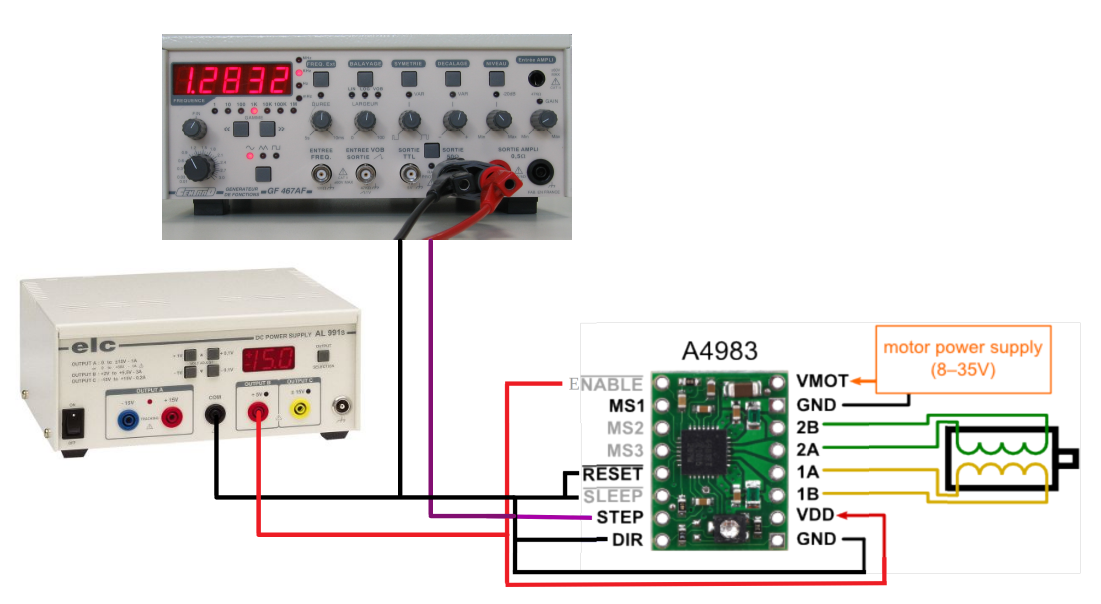
\includegraphics[width=0.8\linewidth]{\figures/sch_a4988.png}
    \decoRule
    \caption[
    Schéma de câblage d'un contrôleur moteur sur la Raspberry Pi]{
    Schéma de câblage d'un contrôleur moteur sur la Raspberry Pi}
    \label{fig:Schéma de câblage d'un contrôleur moteur sur la Raspberry Pi}
    \end{figure}

Durant ce test nous avons vérifié le bon fonctionnement du moteur et contrôleur moteur.

Pour nous assurer que les moteurs de rotation et inclinaison sont suffisamment coupleux et résistant nous avons placé une courroie autour de l'axe du moteur et au bout de cette dernière nous avons attaché une masse d'environ $10kg$.
Ce test fut un succès et nous avons validé le choix des moteurs.

\begin{figure}[H]
    \centering
    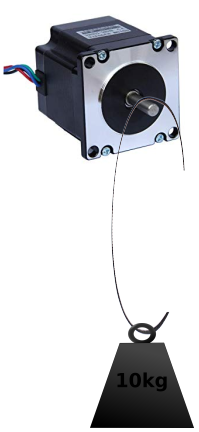
\includegraphics[width=0.3\linewidth]{\figures/sch_test_motor.png}
    \decoRule
    \caption[
    Test de la puissance du moteur]{
    Test de la puissance du moteur}
    \label{fig:Test de la puissance du moteur}
    \end{figure}

Nous avons profité du test pour manuellement utiliser les modes de pas en appliquant aux entrées MS1, MS2, MS3 du $5V$ en suivant la documentation ci-dessous~:

\begin{figure}[H]
    \centering
    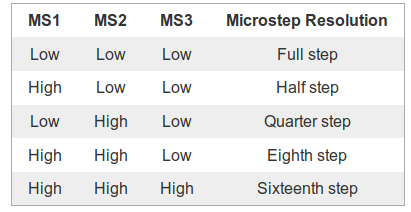
\includegraphics[width=0.5\linewidth]{\figures/tab_a4988_ms.png}
    \decoRule
    \caption[
    Documentation microStep a4988]{
    Documentation microStep a4988}
    \label{fig:Documentation microStep a4988}
    \end{figure}

